
    % \item 
    % Polynomials give rise to ramified coverings.
    % Let $p(z)$ be a non-constant polynomial over the complex numbers. 
    % \begin{itemize}
    %     \item A \emph{ramified value} of $p$ is a complex number $c$ such that the polynomial $p(z) = c$ has multiple roots. Show that the set of ramified values for any polynomial is finite. (Hint: look at $p'(z)$.)
    %     \item A \emph{ramified point} of $p$ is a complex number $z$ such that $p(z)$ is a ramified value. Show that the set of ramified values is finite.
    %     \item Let $U$ denote the set of unramified points and let $V$ denote the set of all unramified values. 
    %     The polynomial $p$ naturally restricts to a map $p: U \to V$. 
    %     Show that $p$ is a covering map. 
    %     You can assume the fact that inverse of any bijective holomorphic function is also holomorphic.
    %  \end{itemize}
        
        \item Orientation of simplices.
    Let $X$ be a topological space.
    Let $[v_0 v_1 v_2]$ denote a singular chain $\sigma : | \Delta ^2 | \to X$.
    \begin{enumerate}
        \item Show that 
        $[v_0 v_1 v_2] - [v_2 v_1 v_0]$ is exact.
        \item Show that
        $[v_0 v_1 v_2] + [v_1 v_0 v_2]$ is exact.
        \item Conclude that for any permutation $\sigma$ of the set $ \{0, 1 , 2\}$ 
        \begin{align*}
            [v_0 v_1 v_2] - {sign(\sigma)} \cdot [v_{\sigma(0)} v_{\sigma(1)} v_{\sigma(2)}]
        \end{align*}
        is exact.
    \end{enumerate}
     Because of this proposition you can freely \emph{reorient}
        
            \item (optional) Klein bottle.
    \begin{figure}[h]
        \centering
        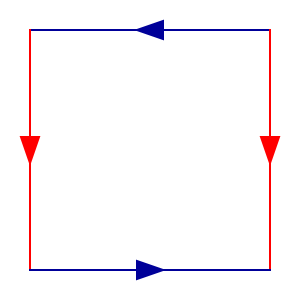
\includegraphics[width=100px]{images/klein-bottle.png}
        \caption{Gluing diagram of a Klein-bottle.}
    \end{figure} 
         
        \item Direct sums of chain complexes


    \item In a category $\mathbf{C}$, the pushout of morphisms $f: A \to B$ and $g : A \to C$ 
    \begin{center}
        \begin{tikzcd}
            A \arrow["f", r] \arrow["g", d, swap]  & B \\
            C
        \end{tikzcd}
    \end{center}
    is an object $D$ and two morphisms $f': B \to D'$ and $g' : C \to D'$ such that
    \begin{itemize}
        \item the following diagram commutes
        \begin{center}
            \begin{tikzcd}
                A \arrow["f", r] \arrow["g", d, swap]  & B  \arrow["f'", d] \\
                C \arrow["g'", r, swap] & D',
            \end{tikzcd}
        \end{center}
        \item 
        and for every $(D'',f'': B \to D'', g'': C \to D'')$ such that the following diagram commutes
        \begin{center}
            \begin{tikzcd}
                A \arrow["f", r] \arrow["g", d, swap]  & B  \arrow["f''", d] \\
                C \arrow["g''", r, swap] & D''
            \end{tikzcd}
        \end{center}
        \item and there exists a unique map $u: D' \to D''$ such that the following diagram commutes
        \begin{center}
            \begin{tikzcd}
                A \arrow["f", r] \arrow["g", d, swap]  
                    & B  \arrow["f'", d] \arrow["f''", ddr, bend left] \\
                C \arrow["g'", r, swap] \arrow["g''", drr, bend right, swap]
                    & D' \arrow["\exists ! u", dr, dashed] \\
                & & D''.
            \end{tikzcd}
        \end{center}    
    \end{itemize} 
    
    \begin{enumerate}
        \item Let $(X,x)$ be a space in $\mathbf{Top}_*$ and let $U$ and $V$ be open subsets of $X$ such that $x \in U \cap V$.
        Show that the pushout of the inclusions $j_U: U \cap V \to U$ and $j_V:U \cap V \to V$ in $\mathbf{Top}_*$ is ($U \cup V$, $i_U: U \to U \cup V$, $i_V: V \to U \cup V$).
        \begin{center}
        \begin{tikzcd}
            U \cap V \arrow["j_U", r] \arrow["j_V", d, swap]  
                & U  \arrow["i_U", d] \arrow["\varphi", ddr, bend left] \\
            V \arrow["i_V", r, swap] \arrow["\psi", drr, bend right, swap]
                & U \cup V \arrow["\exists !", dr, dashed] \\
            & & Y.
        \end{tikzcd}
        \end{center}
        \item Let $A, B, C$ be groups. Show that the pushout of group homomorphisms  $f: A \to B$ and $g : A \to C$ in $\mathbf{Groups}$ is ($B * C / N$, $f':B \to B*C/N$, $g':C \to B*C/N$) , where $N(A)$ is the smallest normal subgroup of $B *C$ generated by the elements $f(a)^{-1} g(a)$ for all $a \in A$, and $f'$ and $g'$ send elements of $B$ and $C$, respectively, to single letter words.
        \begin{center}
        \begin{tikzcd}
            A \arrow["f", r] \arrow["g", d, swap]  
                & B  \arrow["f'", d] \arrow["f''", ddr, bend left] \\
            C \arrow["g'", r, swap] \arrow["g''", drr, bend right, swap]
                & B * C / N \arrow["\exists ! u", dr, dashed] \\
            & & D''.
        \end{tikzcd}
        \end{center}    
        Thus the Seifert--van Kampen theorem says that $\pi_1: \mathbf{Top}_* \to \mathbf{Groups}$ preserves certain kinds of pushouts.\footnote{See also \url{https://math.stackexchange.com/questions/985606/what-categorical-limits-and-colimits-does-pi-1-preserve}.}
    \end{enumerate}